\chapterimage{orange2.jpg}
\chapterspaceabove{6.75cm} 
\chapterspacebelow{7.25cm} 
\chapter{Preliminary Number Theory and Cryptography}
%intro
In this chapter, we will look into one of the most exciting part of mathematics, and it is also a
crucial cornerstone for computer science. The inception of number theory can be traced back to ancient civilizations, but it began to emerge as a distinct mathematical discipline with the work of the Greek mathematician Euclid. His monumental work, "Elements," laid the groundwork for the study of prime numbers and proved fundamental theorems, such as the infinitude of primes, which are still central to number theory today. The nature of whole numbers, especially the intriguing properties of prime numbers—the building blocks of all natural numbers—has fascinated mathematicians for centuries. Over time, the field has expanded to include a rich array of topics such as the distribution of primes, the solutions of Diophantine equations, modular arithmetic, and the exploration of number-theoretic functions like the Riemann zeta function. Number theory's initial focus on prime numbers and divisibility has blossomed into a diverse and vibrant branch of mathematics, with applications ranging from cryptography to the theory of chaos.

\section{Divisibility and Modular Arithmetic}
We start with the divisibility of number, as it is the basis of many further topics.
Divisibility serves as the cornerstone of number theory due to several pivotal reasons. It is the bedrock upon which the Fundamental Theorem of Arithmetic stands, declaring that each integer greater than 1 is uniquely decomposable into a product of prime numbers. These primes are the elemental units, akin to atoms in chemistry, from which all other numbers are constructed. The concepts of greatest common divisors and least common multiples emerge from divisibility, forming the basis of crucial algebraic structures such as rings and fields, and thereby extending number theory into algebraic realms. Furthermore, the pursuit of integer solutions to equations, known as Diophantine analysis, is deeply reliant on principles of divisibility. In the modern context, divisibility underpins cryptographic systems, leveraging the challenging task of prime factorization to secure digital communication. Moreover, divisibility naturally extends to modular arithmetic, enriching number theory with the study of congruences, which has profound implications across mathematics and its myriad applications. Therefore, the study of divisibility is not just foundational but also a connective thread that weaves through the entire fabric of number theory.

\subsection{Division and Divisibility}
To figure out problems related to \textbf{Divisibility}, we must figure out the definition and properties
of \textbf{Division}. We were taught in the primary school that a division is an operation  that
divides a number to a certain part. For instance, $6\div2=3$, and $6\div4=1.5$. Sometimes, the
division produce an integer as result, while sometimes not. We define division as follows:
    \begin{definition}[Division]
        The division of a number \( a \) by a non-zero number \( b \) is denoted by \( a \div b \) or \( \frac{a}{b} \), and it gives the quotient \( q \) and possibly a remainder \( r \). The operation can be written as:
        \[
        a = b \times q + r
        \]
        where \( 0 \leq r < b \) and \(q \in \mathbb{Z}\).
    \end{definition}
    In $6\div2=3$, clearly we have $6=2\times3+0$, with $r=0$, $q=3$. But how could we explain
    $6\div4=1.5$? The quotient is a decimal instead of an integer. Fundamentally, we cannot separate
    the number 6 in to 4 parts to be represented as integer. In this case the division can be represented
    as $6 = 4\times0+6$, meaning $q=0$ and $r=6$. Actually, $6\div4=1.5$ is not defined as only
    division, but \textbf{True Division}.
    \begin{definition}[True Division]
        True division is concerned with the quotient including the remainder as a fractional part. In true division, when \( a \) is divided by \( b \), the quotient \( q \) is a real number that can be represented as:
        \[
        q = \frac{a}{b}
        \]
    \end{definition}
    You may find that true division doesn't have a remainder. This is just because the purpose of 
    these two operations are different, as true division only focus on the scale of each part of
    $a$, but division involves the divisibility and remainder, which will be discussed further
    in this chapter.

    Now that we have defined division and true division, you may understand the following definition
    of divisibility easier.
    \begin{definition}[Divisibility]
        If $a$ and $b$ are integers with $a \neq 0$, we say that $a$ divides $b$ if there is an integer $c$ such that $b = a\times c$ (or equivalently, if $b$ a is an integer). When $a$ divides $b$ we say that $a$ is a factor or divisor of $b$, and that $b$ is a multiple of $a$. The notation a $\mid$ b denotes that $a$ divides $b$. We write $a \nmid b$ when $a$ does not divide $b$
    \end{definition}
    For example, we have $4\mid 20$, because $20\div4$ gives an integer, however, $4\nmid 21$, as the answer
    cannot be represented as integer. Besides, we have:
    \begin{equation}
        a\mid b \iff \exists c(ac=b).
    \end{equation}

    \begin{problem}
        Let \( n \) and \( d \) be positive integers. How many positive integers not exceeding \( n \) are divisible by \( d \)?
    \end{problem}
    \textbf{Solution:} The positive integers divisible by \( d \) are all the integers of the form \( dk \), where \( k \) is a positive integer. Hence, the number of positive integers divisible by \( d \) that do not exceed \( n \) equals the number of integers \( k \) with \( 0 < dk \leq n \), or with \( 0 < k \leq \frac{n}{d} \). Therefore, there are \( \left\lfloor \frac{n}{d} \right\rfloor \) positive integers not exceeding \( n \) that are divisible by \( d \).

    Divisibility holds the following properties, which could be proven directly.
    \begin{theorem}[Properties of Divisibility] \label{Properties of Divisibility}
        Let $a$, $b$, and $c$ be integers, where $a\neq 0$, then:
        \begin{enumerate}
            \item if $a \mid b$ and $a \mid c$, then $a \mid (b+c)$
            \item if $a \mid b$ then $a \mid bc$ for all integers $c$
            \item if $a \mid b$ and $b\mid c$, then $a \mid c$
        \end{enumerate}
    \end{theorem}
    \begin{proof}
        Since \( a \mid b \) and \( a \mid c \), there exist integers \( m \) and \( n \) such that \( b = am \) and \( c = an \). Therefore, \( b+c = am + an = a(m+n) \), and since \( m+n \) is an integer, it follows that \( a \mid (b+c) \).
        
        Given \( a \mid b \), there exists an integer \( k \) such that \( b = ak \). For any integer \( c \), \( bc = a(kc) \). Since \( kc \) is an integer (because the product of two integers is an integer), \( a \mid bc \).
        
        If \( a \mid b \) and \( b \mid c \), then there exist integers \( p \) and \( q \) such that \( b = ap \) and \( c = bq \). Substituting the expression for \( b \) into the equation for \( c \) gives \( c = (ap)q = a(pq) \). Since \( pq \) is an integer, \( a \mid c \).
    \end{proof}
    With this we have the following conclusion.
    \begin{corollary}\label{div1}
        if $a$, $b$, and $c$ are integers, where $a\neq 0$, such that $a\mid b$ and $a\mid c$, then $a\mid mb + nc$ whenever $m$ and $n$ are integers.
    \end{corollary}
    This could be proven in direct proof, which you will finish in the exercise.

    \subsection{Modular Arithmetic}
    In this section, we will focus on the remainder of division, as well as modular arithmetic.
    In the definition of division, we involved $q$ and $r$, which denotes the quotient and
    the remainder of the operation. We use the following notations to denote each of both.
    \begin{notation}[div and mod]
        For $a$, $b\in \mathbb{R}$.
        $a = b\times q + r$    
        $$q = a\ \text{\textbf{div}}\ b$$
        $$r = a\ \text{\textbf{mod}}\ b$$
    \end{notation}
    Besides, when $a$ is an integer and $b$ is a positive integer, we have $a\ \text{\textbf{div}}\ b = \left \lfloor  a/b \right \rfloor$.
    \begin{example}
        What are the quotient and remainder when 93 is divided by 9?
    \end{example}
    \textbf{Solution:} $93 = 9\times 10 + 3$. $q = 10$, $r = 3$.

    The quotient is $93\ \textbf{div}\ 9 = 10 = \lfloor93/9\rfloor = \lfloor10.3333\dots \rfloor = 10$

    The remainder is $93\ \textbf{mod}\ 9 = 3 = 93 - 90$
    
    \begin{example}
        What are the quotient and remainder when -93 is divided by 9?
    \end{example}
    \textbf{Solution:} $-93 = 9\times (-11) + 6$. $q = -11$, $r = 6$.
    
    Remember that we must make sure $r\geq0$ as we defined earlier, even though $-93 = 9\times(-10) - 3$.
    But remainder could be positive in other division algorithm, which we will discuss in the exercise.

    We have already introduced the notation $ a\ \textbf{mod}\ m $ to represent the remainder when an integer
    $a$ is divided by the positive integer $m$. We now introduce a different, but related, notation
    that indicates that two integers have the same remainder when they are divided by the positive
    integer $m$. But why we need to find and study the numbers with the same remainder by dividing 
    the same positive integer? Studying numbers that yield the same remainder when divided by a given positive integer is a
    fundamental part of number theory; later you will understand why say so.
    \begin{definition}
        If $a$ and $b$ are integers and $m$ is a positive integer, then $a$ is \textbf{congruent} 
        to $b$ \textbf{modulo} $m$ if $m$ divides $a - b$. 
        We use the notation $a \equiv b (\bmod m)$ to indicate that $a$ is congruent to $b$ modulo 
        $m$. We say that $a \equiv b (\bmod m)$ is a congruence and that $m$ is its modulus 
        (plural moduli). If $a$ and $b$ are not congruent modulo $m$, we write $a \not\equiv b (\bmod m)$.
    \end{definition}
    Do note that mod and \textbf{mod} are different notations. The first represents a relation on the set of integers, whereas the
    second represents a function. However, they are still related.
    \begin{theorem}
        Let $a$ and $b$ be integers, and let $m$ be a positive integer. $a \equiv b (\bmod \  m)$ if and only if $a\ \textbf{mod}\ m$ = $b\ \textbf{mod}\ m$.
    \end{theorem}
    \begin{proof}
        First, suppose \( a \equiv b \pmod{m} \). By definition of congruence modulo \( m \), \( m \) divides \( a - b \), which means there exists some integer \( k \) such that \( a - b = km \).

        Dividing \( a \) and \( b \) by \( m \), they both leave the same remainder \( r \), since \( a = q_1m + r \) and \( b = q_2m + r \) for some integers \( q_1 \) and \( q_2 \). The remainder \( r \) in both cases is the same because the difference \( a - b \) is a multiple of \( m \), which does not affect the remainder.

        Conversely, if \( a \mod m = b \mod m \), then both \( a \) and \( b \) leave the same remainder when divided by \( m \). Denote this common remainder as \( r \).

        We can write \( a = q_1m + r \) and \( b = q_2m + r \) for some integers \( q_1 \) and \( q_2 \). Subtracting these two equations, we get \( a - b = (q_1 - q_2)m \), which shows that \( a - b \) is a multiple of \( m \).

        Therefore, \( m \) divides \( a - b \), and by definition of congruence modulo \( m \), we have \( a \equiv b \pmod{m} \).

        This completes the proof.
    \end{proof}
    \begin{remark}
        Remember, when we say if and only if, we need proof from each of the both statements to the other.
    \end{remark}
    \begin{theorem}\label{mod2}
        Let $m$ be a positive integer. The integers $a$ and $b$ are congruent modulo $m$ if and only if there is an integer $k$ such that $a = b + km$.
    \end{theorem}
    The proof is similar and not complex, try to prove it in the exercise.

    \begin{theorem}
        Let $m$ be a positive integer. If $a \equiv b \pmod{m}$ and $c \equiv d \pmod{m}$, then
        \begin{equation*}
            a + c \equiv b + d \pmod{m}
        \end{equation*}
        and
        \begin{equation*}
            ac \equiv bd \pmod{m}.
        \end{equation*}
        \end{theorem}
        
        \begin{proof}
        We use a direct proof. Because $a \equiv b \pmod{m}$ and $c \equiv d \pmod{m}$, by Theorem 4 there are integers $s$ and $t$ with $b = a + sm$ and $d = c + tm$. Hence,
        \begin{align*}
            b + d &= (a + sm) + (c + tm) = (a + c) + m(s + t)
        \end{align*}
        and
        \begin{align*}
            bd &= (a + sm)(c + tm) = ac + m(at + cs + stm).
        \end{align*}
        Hence,
        \begin{equation*}
            a + c \equiv b + d \pmod{m}
        \end{equation*}
        and
        \begin{equation*}
            ac \equiv bd \pmod{m}.
        \end{equation*}
        \end{proof}
        
        \begin{example}
        Because $7 \equiv 2 \pmod{5}$ and $11 \equiv 1 \pmod{5}$, it follows that
        \begin{equation*}
            18 = 7 + 11 \equiv 2 + 1 = 3 \pmod{5}
        \end{equation*}
        and that
        \begin{equation*}
            77 = 7 \cdot 11 \equiv 2 \cdot 1 = 2 \pmod{5}.
        \end{equation*}
        \end{example}

        \begin{corollary}
            Let $m$ be a positive integer and let $a$ and $b$ be integers. Then
            \begin{equation*}
                (a + b) \bmod m = ((a \bmod m) + (b \bmod m)) \bmod m
            \end{equation*}
            and
            \begin{equation*}
                ab \bmod m = ((a \bmod m)(b \bmod m)) \bmod m.
            \end{equation*}
            \end{corollary}
            
            \begin{proof}
            By the definitions of $\bmod$ and of congruence modulo $m$, we know that $a \equiv (a \bmod m) \pmod{m}$ and $b \equiv (b \bmod m) \pmod{m}$. Hence,
            \begin{equation*}
                a + b \equiv (a \bmod m) + (b \bmod m) \pmod{m}
            \end{equation*}
            and
            \begin{equation*}
                ab \equiv (a \bmod m)(b \bmod m) \pmod{m}.
            \end{equation*}
            The equalities in this corollary follow from these last two congruence.
            \end{proof}

            We can define arithmetic operations on \( \mathbb{Z}_m \), the set of nonnegative integers less than \( m \), that is, the set \( \{0, 1, \ldots, m - 1\} \). In particular, we define addition of these integers, denoted by \( \oplus_m \), by
        \[
        a \oplus_m b = (a + b) \bmod m,
        \]
        where the addition on the right-hand side of this equation is the ordinary addition of integers, and we define multiplication of these integers, denoted by \( \odot_m \), by
        \[
        a \odot_m b = (a \cdot b) \bmod m,
        \]
        where the multiplication on the right-hand side of this equation is the ordinary multiplication of integers. The operations \( \oplus_m \) and \( \odot_m \) are called addition and multiplication modulo \( m \) and when we use these operations, we are said to be doing arithmetic modulo \( m \).

        \begin{example}
        Use the definition of addition and multiplication in \( \mathbb{Z}_m \) to find \( 7 \oplus_{11} 9 \) and \( 7 \odot_{11} 9 \).

        \textbf{Solution:} Using the definition of addition modulo 11, we find that
        \[
        7 \oplus_{11} 9 = (7 + 9) \bmod 11 = 16 \bmod 11 = 5,
        \]
        and
        \[
        7 \odot_{11} 9 = (7 \cdot 9) \bmod 11 = 63 \bmod 11 = 8.
        \]
        Hence, \( 7 \oplus_{11} 9 = 5 \) and \( 7 \odot_{11} 9 = 8 \).
        \end{example}
        \begin{remark}
            sometimes, normal notations are also used to express this calculation with subscript.
        \end{remark}


    \subsection{Exercises}
    \begin{exercise}
        Prove corollary \ref{div1} that if $a$, $b$, and $c$ are integers, where $a\neq 0$, such that $a\mid b$ and $a\mid c$, then $a\mid mb + nc$ whenever $m$ and $n$ are integers.
    \end{exercise}
    \begin{proof}
        By theorem \ref{Properties of Divisibility}, $a\mid b$ and $a\mid c$ gives us $a\mid mb$
        and $a\mid nc$ (property 2). Hence, $a\mid (mb+nc)$ (property 1). This completes the proof.
    \end{proof}
    
    \begin{exercise}
        floored division he truncated division
    \end{exercise}

    \begin{exercise}
        Prove theorem \ref{mod2}, you may use other theorems or corollary in this chapter.
    \end{exercise}
    \begin{proof}
        If $a \equiv b (\bmod \ m)$, that means we have $m\mid(a-b)$. There must be a integer $k$, such that $a = b + km$ (theorem \ref{mod2}). Conversely, if we have a integer $k$, such that $a = b+km$, we have $km = a-b$. Hence, $m\mid(a-b)$, $a \equiv b (\bmod \ m)$.
    \end{proof}
    \begin{exercise}
        show that for integer $\displaystyle a,\ b,\ c\ \in \mathbb{Z}^{+}$, $\displaystyle a,c\neq 0$ and $\displaystyle ac\mid bc,$then $\displaystyle a\mid b$.
    \end{exercise}
    \begin{proof}
        $\displaystyle ac\mid bc$ means that $\displaystyle bc=k( ac)$ for some integer $\displaystyle k$, so we have $\displaystyle b=ka$, this means $\displaystyle a\mid b$.
    \end{proof}
    \begin{exercise}
        Prove that if $\displaystyle a$ and $\displaystyle b$ are integers and $\displaystyle a$ divides $\displaystyle b$, then $\displaystyle a$ is odd or $\displaystyle b$ is even.
    \end{exercise}
    \begin{proof}
        We could try proof by contrapositive. Suppose for $\displaystyle a$ is even and $\displaystyle b$ is odd, 
        $\displaystyle a,b\in \mathbb{Z} ,\ a\mid b$. Then $\displaystyle b=ka$ for some integer $\displaystyle k$. 
        Make $\displaystyle a=2n,\ b=2n+1,\ n\in \mathbb{Z}$, then there should be $\displaystyle 2n+1=2kn$. 
        However, in this case we have $\displaystyle k=\frac{2n+1}{2n}$, meaning that $\displaystyle k$ is not an 
        integer, which contradict the assumption. This completes the proof.
    \end{proof}
    \begin{exercise}
        Prove that if $a$ is a positive integer, then $4\nmid (a^2+2)$.
    \end{exercise}
    \begin{proof}
        Consider any positive integer $a$. We know that $a$ can be expressed in one of the following forms where $n$ is an integer:
        \begin{itemize}
            \item $a = 4n$
            \item $a = 4n + 1$
            \item $a = 4n + 2$
            \item $a = 4n + 3$
        \end{itemize}
        Now, we examine $a^2$ modulo 4 for each case:
        \begin{align*}
            (4n)^2 &= 16n^2 = 4 \cdot 4n^2 \equiv 0 \pmod{4}, \\
            (4n + 1)^2 &= 16n^2 + 8n + 1 = 4(4n^2 + 2n) + 1 \equiv 1 \pmod{4}, \\
            (4n + 2)^2 &= 16n^2 + 16n + 4 = 4(4n^2 + 4n + 1) \equiv 0 \pmod{4}, \\
            (4n + 3)^2 &= 16n^2 + 24n + 9 = 4(4n^2 + 6n + 2) + 1 \equiv 1 \pmod{4}.
        \end{align*}
        Adding 2 to $a^2$ in each case yields:
        \begin{align*}
            a^2 + 2 &\equiv 2 \pmod{4} \quad \text{if } a^2 \equiv 0 \pmod{4}, \\
            a^2 + 2 &\equiv 3 \pmod{4} \quad \text{if } a^2 \equiv 1 \pmod{4}.
        \end{align*}
        In both cases, $a^2 + 2$ does not yield a remainder of $0$ modulo $4$. Thus, it cannot be divisible by $4$.

        Therefore, we have proven that for any positive integer $a$, the expression $a^2 + 2$ is not divisible by $4$.
    \end{proof}

    \begin{exercise}
        Suppose that \( a \) and \( b \) are integers, \( a \equiv 11 \mod{19} \), and \( b \equiv 3 \mod{19} \). 
        Find the integer \( c \) with \( 0 \leq c \leq 18 \) such that
        \begin{enumerate}
            \item \( c \equiv 13a \mod{19} \).
            \item \( c \equiv 8b \mod{19} \).
            \item \( c \equiv a - b \mod{19} \).
            \item \( c \equiv 7a + 3b \mod{19} \).
            \item \( c \equiv 2a^2 + 3b^2 \mod{19} \).
            \item \( c \equiv a^3 + 4b^3 \mod{19} \).
        \end{enumerate}
    \end{exercise}

    \textbf{Solution:} This problem is equivalent to asking for the right-hand side mod 19. So we just do the arithmetic and compute the remainder upon division by 19.
    \begin{enumerate}
        \item \( 13 \cdot 11 = 143 \equiv 10 \mod{19} \)
        \item \( 8 \cdot 3 = 24 \equiv 5 \mod{19} \)
        \item \( 11 - 3 = 8 \mod{19} \)
        \item \( 7 \cdot 11 + 3 \cdot 3 = 86 \equiv 10 \mod{19} \)
        \item \( 2 \cdot 11^2 + 3 \cdot 3^2 = 269 \equiv 3 \mod{19} \)
        \item \( 11^3 + 4 \cdot 3^3 = 1439 \equiv 14 \mod{19} \)
    \end{enumerate}

    \begin{exercise}
        Let \( m \) be a positive integer. Show that \( a \mod m = b \mod m \) if \( a \equiv b \pmod{m} \).
    \end{exercise}
    \begin{proof}
        Assume that \( a \equiv b \pmod{m} \). This means that \( m \mid a - b \), say \( a - b = mc \), so that \( a = b + mc \). Now let us compute \( a \mod m \). We know that \( b = qm + r \) for some nonnegative \( r \) less than \( m \) (namely, \( r = b \mod m \)). Therefore, we can write \( a = qm + r + mc = (q + c)m + r \). By definition, this means that \( r \) must also equal \( a \mod m \). That is what we wanted to prove.
    \end{proof}

\section{Number Representations and Algorithms}
    In everyday life, we use decimal notation to express integers. Though this is not
    for all cases, as we are using a 60 base system for time. However, in computer science, binary, octal, and hexadecimal
    systems are widely used for number representation. The reason is that binary system consist of 
    only 0 and 1, as we have mentioned in Boolean algebra, this system is perfect for logic operations
    in side the computer. What's more, 0 and 1 could be easily represented by the on and off of tiny
    switches in the integrated circuits. This chapter looks into the representation of number
    in different bases and their relationship, with a tress on binary representation that computer
    system uses. Meanwhile, we will go through algorithm of some operations between number, and
    analyze them accordingly.
    \subsection{Representations of Numbers and Base Conversion}
    In whichever base, a number could be expressed using the exponent of the base.
    \begin{theorem}[Representation of Number]
		Let $b$ be an integer greater than 1. Then if $n$ is a positive integer, it can be expressed uniquely 
		in the form:\\
		$n=a_{k} b^{k}+a_{k-1} b^{k-1}+\cdots+a_{1} b+a_{0}$\\
		where $k$ is a nonnegative integer, $a_0, a_1,\cdots, a_k$ are negative integers less than b, and $a_k \neq 0$
	\end{theorem}
    For example, 1024 could be interpreted as $1024 = 1\times10^3+\times10^2+2\times10^1+4\times10^0$.
    Besides, the base of number constraints the possible numbers to be used on the bits. For example,
    under decimal system, we cannot take 10 as one digit, instead it is a number with two digits 1 and 0,
    because for bits under decimal system, the maximum only goes to 9. Therefore, you could take it as
    a fact that for a system of base $b$, the biggest value for one bit is $b-1$. Similarly, we see
    only 0 and 1 in binary, 1-7 in ocatl, 1-15 in hexadecimal expression.

    To indicate the base of a number, we use the following subscript.
    \begin{notation}[$xxxx_b$]
        We use $_b$ to show the base of a number, where $b$ is the base number.
    \end{notation}

    The other important fact is that numbers are just numbers, base is only the way we gauge them.
    However you change $121_{10}$, to whatever base, it is still 121 in decimal, but just expressed 
    in a different way.
    \subsubsection*{Binary, Octal, and Hexadecimal Expression}
    In \textbf{binary expansion}, the base on any integer is 2, that is to say, the number in each digit is either 0 or 1.
We can expand binary integer in the same ways as mentioned in last section.

\begin{example}
	What is the decimal expansion of the integer that has $(101011111)_2$ as its binary expansion?

		$(101011111)_2$ has nine digits, so we have:\\
		$(101011111)_2$ = $1\times 2^9 + 1\times 2^7+1\times 2^5+1\times 2^4+1\times 2^3+1\times 2^2+1\times 2^1+1\times 2^0 = 351$

\end{example}
Decimal expansion of octal expansions could be calculated in the same way as the binary expansion. However, 
Sixteen different digits are required for hexadecimal expansions. Usually, the hexadecimal digits used are 
0, 1, 2, 3, 4, 5, 6, 7, 8, 9, A, B, C, D, E, and F, where the letters A through F represent the digits 
corresponding to the numbers 10 through 15 (in decimal notation). 
\begin{example}
	What is the decimal expansion of the number with hexadecimal expansion $(2AE0B)_{16}$?
\end{example}
In hexadecimal cases, the only difference is that capital latters are used to represent two-digit number in
		one digit. We still have:\\
		$(2AE0B)_{16}$ = $2\times 16^4 + 10\times 16^3 + 14\times 16^2 + 0 \times 16^1 + 11 \times 16^0=175627$

        \textbf{NOTICE: } Each hexadecimal digit can be represented using four bits. For instance, 
we see that $(1110 0101)_2$ = $(E5)_{16}$ because $(1110)_2$ = $(E)_{16}$ and $(0101)_2 = (5)_{16}$. Bytes, which are bit strings 
of length eight, can be represented by two hexadecimal digits.

    \subsection{Base Conversion}
    \subsubsection*{Base conversion of Integer}
    Now we have learned how to express numbers in different base systems, but is there any way to
    convert them from one base to the other? You may have realized that a general solution is to
    convert the number back to decimal form, and then to the target base. Yes, it works, but can we
    make it better? One way to this is to use the general base conversion algorithm.
    The most common algorithm to constructing the base $b$ expansion of an integer n is as follows:\\
First, divide $n$ by $b$ to obtain a quotient and remainder, that is: \\
\begin{center}
	$\displaystyle n\ =\ bq_{0} \ +\ a_{0} \ \ \ \ \ \ \ \ \ \ \ \ \ \ \ \ \ \ \ \ \ ( 0\ \leq \ a_{0} \ < \ b)$
\end{center}
The remainder, $a_0$, is the rightmost digit in the base b expansion of $n$. Next, divide $q_0$ by $b$ toobtain:\\
\begin{center}
	$\displaystyle q_0\ =\ bq_{1} \ +\ a_{1} \ \ \ \ \ \ \ \ \ \ \ \ \ \ \ \ \ \ \ \ \ ( 0\ \leq \ a_{1} \ < \ b)$
\end{center}
We see that $a_1$ is the second digit from the right in the base b expansion of n. Then, we just continue this process
until we obtain a quotient equal to zero. This algorithm produces the base $b$ digits of $n$ from the right to the left.

\begin{example}
	Find the hexadecimal expansion of $(177130)_{10}$.
		\begin{center}
		$177130 = 16 \cdot 11070 + 10$\\
		$11070 = 16 \cdot 691 + 14$\\
		$691 = 16 \cdot 43 + 3$\\
		$43 = 16 \cdot 2 + 11$\\
		$2 = 16 \cdot 0 + 2 $\\
		\end{center}
		Therefore, $(177130)_{10} = (2B3EA)_{16}$
\end{example}
    This method is equivalent to the following pseudocode.
    \begin{algorithm}
        \caption{Base conversion of an integer $n$ to base $b$}
        \begin{algorithmic}[H]
        \Require{An integer $n$ and a base $b$ to convert to}
        \Ensure{The base $b$ expansion of $n$}
        \Function{ConvertToBase}{$n, b$}
            \State $digits \gets$ empty list
            \While{$n > 0$}
                \State $remainder \gets n \bmod b$
                \State Append $remainder$ to $digits$
                \State $n \gets \left\lfloor n / b \right\rfloor$
            \EndWhile
            \State $digits \gets$ reverse $digits$
            \State \textbf{return} $digits$
        \EndFunction
        \end{algorithmic}
        \end{algorithm}
    \subsubsection*{Base Conversion of Float}
    The previous algorithm only deals with integers, so we need a different approach for decimals.
    The algorithm for converting a floating-point number from base 10 to base $b$ is given as follows:

\begin{algorithm}
\caption{Convert a floating-point number to a different base}
\begin{algorithmic}[H]
\Function{ConvertFloatToBase}{$number$, $targetBase$}
    \State $integerPart \gets \lfloor number \rfloor$
    \State $fractionalPart \gets number - integerPart$
    \State $baseInteger \gets \Call{ConvertIntegerToBase}{integerPart, targetBase}$
    \State $baseFraction \gets ``"$
    \While{$fractionalPart > 0$ \textbf{and} length of $baseFraction$ is less than limit}
        \State $fractionalPart \gets fractionalPart \times targetBase$
        \State $baseFraction \gets baseFraction + \lfloor fractionalPart \rfloor$
        \State $fractionalPart \gets fractionalPart - \lfloor fractionalPart \rfloor$
    \EndWhile
    \State \Return $baseInteger + ``." + baseFraction$
\EndFunction
\end{algorithmic}
\end{algorithm}

\begin{example}
Convert the floating-point number 12.375 from base 10 to base 2.
\begin{itemize}
\item Integer part: 12 in base 10 is 1100 in base 2.
\item Fractional part: 0.375 in base 10 to base 2.
\begin{align*}
0.375 \times 2 &= 0.75 \rightarrow \text{integer part is 0} \\
0.75 \times 2 &= 1.5 \rightarrow \text{integer part is 1} \\
0.5 \times 2 &= 1 \rightarrow \text{integer part is 1} \\
\end{align*}
\item The fractional part in base 2 is .011.
\end{itemize}

Therefore, $12.375_{10}$ is $1100.011_{2}$.
\end{example}
Also, when a number consist of both integer and decimal parts, we just deal with them separately
and them put them back together later. You will see these exercises in the problem set.

\subsubsection*{Base Conversion between Binary, Octal, and Hexadecimal number}
The base conversion between Binary, Octal and Hexadecimal numbers are much easier.
\begin{figure}[H]
	\centering
	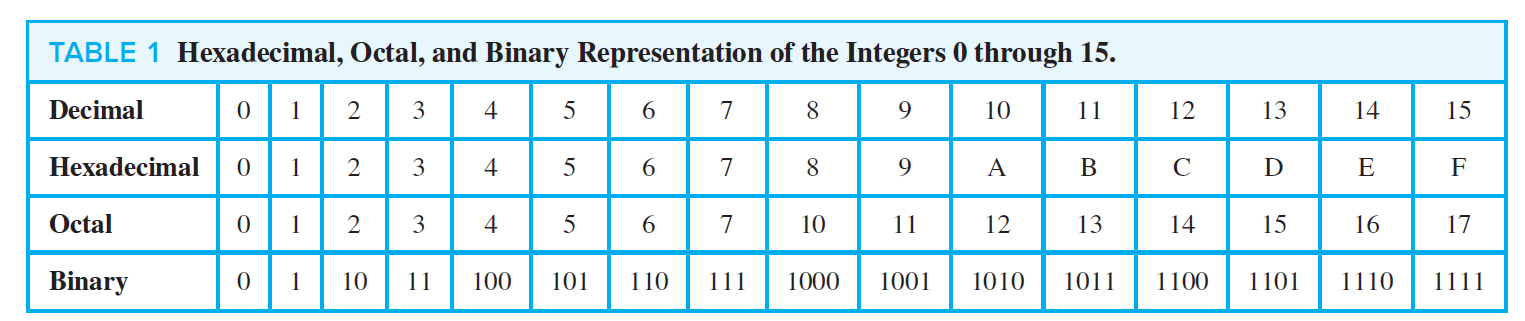
\includegraphics[width=1\linewidth]{converttab.png}
    \caption{Binary, Octal and Hexadecimal Representation}
\end{figure}
The conversion between binary, octal, and hexadecimal systems is straightforward because the bases of these systems (2 for binary, 8 for octal, and 16 for hexadecimal) are related by powers of 2. Specifically:
\begin{itemize}
    \item Octal digits correspond to three binary digits since \(8 = 2^3\). Each octal digit can be directly mapped to a unique combination of three binary bits.
    \item Hexadecimal digits correspond to four binary digits since \(16 = 2^4\). Each hexadecimal digit can be directly mapped to a unique combination of four binary bits.
\end{itemize}
This relationship allows for simple grouping of binary bits into sets of three or four to convert 
to octal or hexadecimal, respectively, without any complex calculation or division. 
\begin{example}
	Find the octal and hexadecimal expansions of $(11\ 1110\ 1011\  1100)_2$ and the binary expansions of $(765)_{8}$ and $(A8D)_{16}$.
\end{example}
\textbf{Solution:} To convert $(11\ 1110\ 1011\  1100)_2$ into octal notation we group the binary digits
into blocks of three, adding initial zeros at the start of the leftmost block if necessary.
These blocks, from left to right, are 011, 111, 010, 111, and 100, corresponding to 3, 7, 2, 7, and 4 respectively. Consequently, we get $(11\ 1110\ 1011\  1100)_2 = (37274)_8$
\par We do the hexadecimal convention in the same way. These blocks, from left to right, are 0011,
1110, 1011, and 1100, corresponding to the hexadecimal digits 3, E, B, and C, respectively. Consequently, $(11\ 1110\ 1011\  1100)_2 = (3EBC)_{16}$
\par \textbf{NOTE: } The conversion could be done inversely in the same way. If the number of bit is not the multiple of 4 when you are converting between 2 and 16 base
number, fill those missing digits/bits with 0.

Whether you noticed or that the base conversion, essentially, is about division and modular arithmetic
that we just learned? The general base conversion algorithm could be simplified to the following algorithm,
where $n$ denotes the number to be converted and $b$ is the target base.
\begin{algorithm}
    \caption{Constructing Base \( b \) Expansions}
    \begin{algorithmic}[H]
    \Procedure{base \( b \) expansion}{$n, b$: positive integers with $b > 1$}
    \State $q \gets n$
    \State $k \gets 0$
    \While{$q \neq 0$}
    \State $a_k \gets q \mod b$
    \State $q \gets \lfloor q / b \rfloor$
    \State $k \gets k + 1$
    \EndWhile
    \State \textbf{return} $(a_{k-1}, \ldots, a_1, a_0)$ \Comment{The base \( b \) expansion of \( n \)}
    \EndProcedure
    \end{algorithmic}
    \end{algorithm}
    \subsection{Operation Algorithms of Number}
        This section discusses algorithm of basic operation between numbers, of base2. 
        In section, we express the binary number in the form of 
        $$a=(a_{n-1}a_{n-2}\ldots a_1a_0)_2,b=(b_{n-1}b_{n-2}\ldots b_1b_0)_2$$
        where $a$ and $b$ each have n bits.
    \subsubsection*{Addition Algorithm}
    Consider the problem of adding two integers in binary notation. A procedure to perform addition can be based on the usual method for adding numbers with pencil and paper. This method proceeds by adding pairs of binary digits together with carries, when they occur, to compute the sum of two integers. This procedure will now be specified in detail.

    To add \( a \) and \( b \), first add their rightmost bits. This gives
    \[
    a_0 + b_0 = c_0 \cdot 2 + s_0,
    \]
    where \( s_0 \) is the rightmost bit in the binary expansion of \( a + b \) and \( c_0 \) is the carry, which is either 0 or 1. Then add the next pair of bits and the carry,
    \[
    a_1 + b_1 + c_0 = c_1 \cdot 2 + s_1,
    \]
    where \( s_1 \) is the next bit (from the right) in the binary expansion of \( a + b \), and \( c_1 \) is the carry. Continue this process, adding the corresponding bits in the two binary expansions and the carry, to determine the next bit from the right in the binary expansion of \( a + b \). At the last stage, add \( a_{n-1} \), \( b_{n-1} \), and \( c_{n-2} \) to obtain \( c_{n-1} \cdot 2 + s_{n-1} \). The leading bit of the sum is \( s_n = c_{n-1} \). This procedure produces the binary expansion of the sum, namely, \( a + b = (s_n s_{n-1} \ldots s_1 s_0)_2 \).
    Consider the binary addition of two numbers, \( 1011_2 \) and \( 1101_2 \).

The addition process is similar to that used in decimal addition, but it is performed in base 2. Below is the columnar addition process:

\begin{center}
\begin{tabular}{ r >{$}r<{$} }
   & 1011_2 \\
  +& 1101_2 \\
  \hline
   & 11000_2 \\
\end{tabular}
\end{center}

Let's perform the addition step by step:

\begin{enumerate}
    \item Start with the rightmost bits (least significant bits). Add \( 1 + 1 \). Since this is base 2, \( 1 + 1 = 10_2 \). Write down the \( 0 \) and carry the \( 1 \) over to the next column.
    \item Move to the next column. Add \( 1 + 0 + 1 \) (including the carry). This equals \( 10_2 \). Write down the \( 0 \) and carry the \( 1 \).
    \item In the next column, add \( 0 + 1 + 1 \). This equals \( 10_2 \). Write down the \( 0 \) and carry the \( 1 \).
    \item For the leftmost bits (most significant bits), add \( 1 + 1 + 1 \). This equals \( 11_2 \). Write down the \( 1 \) and carry the \( 1 \) to a new column to the left.
    \item Write down the carry.
\end{enumerate}
The final result is \( 11000_2 \).

This algorithm's pseudocode is as listed below.
\begin{algorithm}
    \caption{Addition of Integers}
    \begin{algorithmic}[H]
    \Procedure{add}{$a, b$: positive integers}
    \State {the binary expansions of $a$ and $b$ are $(a_{n-1}a_{n-2}\ldots a_1a_0)_2$}
    \State {and $(b_{n-1}b_{n-2}\ldots b_1b_0)_2$, respectively}
    \State $c \gets 0$
    \For{$j \gets 0$ \textbf{to} $n-1$}
        \State $d \gets \left\lfloor (a_j + b_j + c)/2 \right\rfloor$
        \State $s_j \gets a_j + b_j + c - 2d$
        \State $c \gets d$
    \EndFor
    \State $s_n \gets c$
    \State \textbf{return} $(s_{n}s_{n-1}\ldots s_1s_0)_2$ \Comment{the binary expansion of the sum}
    \EndProcedure
    \end{algorithmic}
    \end{algorithm}

    
    \textbf{Time Complexity:}
    The time complexity of the binary addition algorithm is \( O(n) \), where \( n \) is the number of bits in the binary representation of the inputs.
    \begin{proof}
        Consider the binary addition algorithm which consists of a single loop that iterates \( n \) times, where \( n \) is the number of bits in the binary representations of the two integers being added.
        
        Within the loop, the algorithm performs a constant number of operations for each bit:
        \begin{itemize}
            \item An addition of the \( j \)-th bits of the two numbers \( a_j + b_j \).
            \item An addition of the carry from the previous step \( c \).
            \item A division by 2 to compute the new carry \( d \).
            \item A subtraction to determine the \( j \)-th bit of the sum \( s_j \).
            \item An assignment of the new carry \( c \gets d \).
        \end{itemize}
        
        Since each of these operations has a constant time complexity, and they are all executed once for each bit, the overall time complexity of the loop is linear with respect to the number of bits. Therefore, the time complexity of the entire algorithm is \( O(n) \).
        
        Note that this analysis assumes that basic arithmetic operations (addition, division by 2, subtraction) can be performed in constant time.
        \end{proof}
    \subsubsection*{Multiplication Algorithm}
        Using the same representation of binary number $a$ and $b$, we can define binary multiplication
        as $$\begin{aligned}a b & =a\left(b_{0} 2^{0}+b_{1} 2^{1}+\cdots+b_{n-1} 2^{n-1}\right) \\& =a\left(b_{0} 2^{0}\right)+a\left(b_{1} 2^{1}\right)+\cdots+a\left(b_{n-1} 2^{n-1}\right)\end{aligned}$$.
        The binary multiplication algorithm works similarly to traditional pencil-and-paper multiplication, but with binary digits. Given two binary numbers, we multiply each bit of the second number by the first number, shifting the result left for each subsequent bit.
        \begin{algorithm}
            \caption{Addition of Integers}
            \begin{algorithmic}
            \Procedure{ADD}{$a, b$: positive integers}
                \State {the binary expansions of $a$ and $b$ are $(a_{n-1}a_{n-2}\ldots a_1a_0)_2$}
                \State {and $(b_{n-1}b_{n-2}\ldots b_1b_0)_2$, respectively}
                \State $c \gets 0$
                \For {$j \gets 0 \text{ to } n-1$}
                    \State $d \gets \left\lfloor (a_j + b_j + c)/2 \right\rfloor$
                    \State $s_j \gets a_j + b_j + c - 2d$
                    \State $c \gets d$
                \EndFor
                \State $s_n \gets c$
                \State \Return $(s_{n}s_{n-1}\ldots s_1s_0)_2$ \Comment{the binary expansion of the sum}
            \EndProcedure
            \end{algorithmic}
            \end{algorithm}

        \begin{example}
            \textbf{Find the product of \( a = (110)_2 \) and \( b = (101)_2 \).}
            First note that
            \begin{align*}
            a \cdot b_0 \cdot 2^0 &= (110)_2 \cdot 1 \cdot 2^0 = (110)_2, \\
            a \cdot b_1 \cdot 2^1 &= (110)_2 \cdot 0 \cdot 2^1 = (0000)_2, \\
            \text{and} \\
            a \cdot b_2 \cdot 2^2 &= (110)_2 \cdot 1 \cdot 2^2 = (11000)_2.
            \end{align*}
            To find the product, add \( (110)_2, (0000)_2, \) and \( (11000)_2 \). Carrying out these additions (using Algorithm 2, including initial zero bits when necessary) shows that \( ab = (11110)_2 \).

        \textbf{Time Complexity:} The time complexity of binary multiplication is \(O(n^2)\), where \(n\) is the number of bits in the binary numbers. This is because each bit of one number is multiplied by each bit of the other number, resulting in \(n\) multiplications for each of the \(n\) bits.
        \end{example}
    \subsubsection*{Algorithm for Div and Mod}
        The following algorithm is used to find the quotient and remainder of $a \div b$.
        This is a more general algorithm as it could handle the cases where a is negative
    \begin{algorithm}
        \caption{Computing div and mod.}
        \begin{algorithmic}
        \Procedure{division\_algorithm}{$a$: integer, $d$: positive integer}
            \State $q \gets 0$
            \State $r \gets |a|$
            \While{$r \geq d$}
                \State $r \gets r - d$
                \State $q \gets q + 1$
            \EndWhile
            \If{$a < 0$ \textbf{and} $r > 0$}
                \State $r \gets d - r$
                \State $q \gets -(q + 1)$
            \EndIf
            \State \Return $(q, r)$ \Comment{$q = a \div d$ is the quotient, $r = a \mod d$ is the remainder}
        \EndProcedure
        \end{algorithmic}
        \end{algorithm}
    %\subsection{Modular Exponentiation}

    \subsection{Exercises}


\section{Primes and Greatest Common Divisors}
        In previous chapter, we learned the properties of division and divisibility, as well as
        modular arithmetic. These are the most essential parts of the whole number theory. In this section
        , we will discuss primes and its property. Prime is not something unfamiliar to us, since some may
        even have learned that from the kindergarten or primary school. We will look into the Algorithms
        that could help is find primes and delve into the algebraic properties of prime later. All these
        are foundations of cryptography.
    \subsection{Primes and Related Algorithms}
        To learn prime, of course we need to recap on its definition.
        \begin{definition}[Prime Number]  
            An integer $p$ greater than 1 is called prime if the only positive factors of $p$ are 1 and $p$.
            A positive integer that is greater than 1 and is not prime is called \textbf{composite}.
        \end{definition}    
        Note that, by this definition, 1 is not a prime, as it is only 1 as the only factor.

        The reason why prime numbers are so fascinating to mathematicians is that they have so many
        interesting and unique property, even except for what we have seen in its definition. Below is what we call the fundamental theorem of arithmetic.
        \begin{theorem}[The Fundamental Theorem of Arithmetic]
            For every integer $n > 1$, there exists a unique factorization into prime numbers, up to the order of the factors. Specifically, $n$ can be expressed as
            \[ n = p_1^{a_1} \cdot p_2^{a_2} \cdot \ldots \cdot p_k^{a_k} \]
            where $p_1 < p_2 < \ldots < p_k$ are prime numbers and $a_1, a_2, \ldots, a_k$ are positive integers. This factorization is unique, apart from the order of the prime factors.
        \end{theorem}
        \begin{proof}
            We prove the theorem in two parts: existence and uniqueness.
            
            \textbf{Existence:} We prove by mathematical induction that every integer greater than 1 can be written as a product of primes.
            
            \textit{Base Case:} For $n = 2$, the statement holds true since 2 is itself a prime number.
            
            \textit{Inductive Step:} Assume the statement holds for all integers greater than 1 and less than $n$. Now consider the integer $n$.
            \begin{itemize}
                \item If $n$ is prime, then it is trivially a product of primes (itself).
                \item If $n$ is not prime, it can be written as $n = a \cdot b$ where $1 < a, b < n$. By the inductive hypothesis, both $a$ and $b$ can be factored into a product of primes. Therefore, $n$ can also be expressed as a product of primes by combining the prime factorization of $a$ and $b$.
            \end{itemize}
            This completes the proof of existence.
            
            \textbf{Uniqueness:} Assume, for the sake of contradiction, that there are two distinct prime factorization of $n$:
            \[ n = p_1^{a_1} \cdot p_2^{a_2} \cdot \ldots \cdot p_k^{a_k} = q_1^{b_1} \cdot q_2^{b_2} \cdot \ldots \cdot q_m^{b_m} \]
            where $p_i$ and $q_j$ are prime numbers, and $a_i, b_j$ are positive integers.
            To proceed to the rest of the proof, we need to use Euclid's lemma.

            \textbf{lemma:}

                Let \(p\) be a prime number. If \(p\) divides the product \(ab\), where \(a\) and \(b\) are integers, then \(p\) divides \(a\) or \(p\) divides \(b\).
            \begin{proof}
                Assume \(p\) is a prime that divides \(ab\) but does not divide \(a\). We need to show that \(p\) must divide \(b\).

                Since \(p\) does not divide \(a\), the greatest common divisor (gcd) of \(a\) and \(p\) is 1, i.e., \(\text{gcd}(a, p) = 1\). According to Bezout's identity, there exist integers \(x\) and \(y\) such that:

                \[ax + py = 1\]

                Multiplying both sides of the equation by \(b\), we get:

                \[abx + pby = b\]
                \begin{remark}
                    If this proof is not yet understandable for you, skip it, and check it back after we go over the rest of this chapter about linear combination of primes.
                \end{remark}
                Since \(p\) divides \(ab\) (by assumption), \(p\) divides \(abx\). Also, \(p\) obviously divides \(pby\). Hence, \(p\) divides the sum \(abx + pby\), which means \(p\) divides \(b\).

                This completes the proof, showing that if \(p\) divides \(ab\) and does not divide \(a\), then \(p\) must divide \(b\), in accordance with Euclid's lemma.
            \end{proof}
            By Euclid's lemma, if a prime divides the product of two numbers, it must divide at least one of those numbers. Thus, $p_1$ must divide some $q_j$ on the right-hand side. Since $q_j$ is prime, we conclude that $p_1 = q_j$. Applying this argument symmetrically and repeatedly, we find that each set of prime factors must be identical to the other, contradicting the assumption of two distinct factorization.
            
            Therefore, the prime factorization of any integer greater than 1 is unique, up to the order of the factors, which completes the proof of the Fundamental Theorem of Arithmetic.
            \end{proof}
            
        \begin{example}
            100 can be taken as $100 = 2\cdot 2\cdot 5\cdot 5 = 2^2\cdot 5^2$.
            Both 2 and 5 are primes.
        \end{example}

        Now that we know these interesting properties of prime and its significance, how do we find
        primes, not just correctly, but also efficiently? The most basic algorithm that anyone
        could find is that we can actually check numbers one by one. To find whether an integer $n$ is prime, what we need to do is to check every number from 2 to $n-1$, and use them to divide $n$ one by one. If anyone of them divides $n$, then $n$ is not prime, and vice versa.
        \subsubsection*{Trial Division}
        We actually can apply a more efficient way to determine whether an integer is prime or not.
        Considering the following theorem.
        \begin{theorem}
            If \( n \) is a composite integer, then \( n \) has a prime divisor less than or equal to \( \sqrt{n} \).
        \end{theorem}
        \begin{proof}
            If \( n \) is composite, by the definition of a composite integer, we know that it has a factor \( a \) with \( 1 < a < n \). Hence, by the definition of a factor of a positive integer, we have \( n = ab \), where \( b \) is a positive integer greater than 1. We will show that \( a \leq \sqrt{n} \) or \( b \leq \sqrt{n} \). If \( a > \sqrt{n} \) and \( b > \sqrt{n} \), then \( ab > \sqrt{n} \cdot \sqrt{n} = n \), which is a contradiction. Consequently, \( a \leq \sqrt{n} \) or \( b \leq \sqrt{n} \). Because both \( a \) and \( b \) are divisors of \( n \), we see that \( n \) has a positive divisor not exceeding \( \sqrt{n} \). This divisor is either prime or, by the fundamental theorem of arithmetic, has a prime divisor less than itself. In either case, \( n \) has a prime divisor less than or equal to \( \sqrt{n} \).
            \end{proof}
        Below is the pseudocode for this procedure.
        \begin{algorithm}
            \caption{Primality Test Using Trial Division}
            \begin{algorithmic}[1]
            
            \Function{IsPrime}{$n$}
                \If{$n \leq 1$}
                    \State \Return \textbf{false}
                \EndIf
                \For{$i \gets 2$ \textbf{to} $n-1$}
                    \If{$n \mod i = 0$}
                        \State \Return \textbf{false}
                    \EndIf
                \EndFor
                \State \Return \textbf{true}
            \EndFunction
            
            \end{algorithmic}
            \end{algorithm}
        \begin{example}
            Show that $\sqrt{105}$ is prime.
        \end{example} 
        textbf{Solution:} Primes less than $\sqrt{105}$ are 2, 3, 5, 7. 101 is not divisible
        by any of them, so it is not composite, and thus it is prime.

        We also need an efficient algorithm to factorize a give number to primes. Here is how is
        works. It works as follows.
        \begin{algorithm}
            \caption{Prime Factorization}
            \begin{algorithmic}[H]
            
            \Function{PrimeFactorization}{$n$}
                \State $factors \gets \text{an empty list}$
                \For{$p \gets 2$ \textbf{to} $\infty$}
                    \While{$n \mod p == 0$}
                        \State Add $p$ to $factors$
                        \State $n \gets n / p$
                    \EndWhile
                    \If{$p > n / p$}
                        \State \textbf{break}
                    \EndIf
                \EndFor
                \If{$n > 1$}
                    \State Add $n$ to $factors$
                \EndIf
                \State \Return $factors$
            \EndFunction
            
            \end{algorithmic}
            \end{algorithm}
        \begin{example}
            Find the prime factorization of 8964.
        \end{example}
        \textbf{Solution:}

        \begin{enumerate}
            \item 8964 is even, so start with 2: \( 8964 \div 2 = 4482 \).
            \item 4482 is also even, divide by 2 again: \( 4482 \div 2 = 2241 \).
            \item 2241 is not divisible by 2. The next primes to try are 3, 5, 7, 11, and so on. We find that 2241 is not divisible by any of these primes until we reach 31.
            \item 2241 divided by 31 gives us 71, which is a prime number.
        \end{enumerate}
        
        Thus, the prime factorization of 8964 is \( 2 \times 2 \times 31 \times 71 \), or in exponent form, \( 2^2 \times 31 \times 71 \).

        There are also other method to finding prime numbers or tell whether a number is prime or not. If you are willing
        to delve into it, you may check \href{https://en.wikipedia.org/wiki/Sieve_of_Eratosthenes}{Sieve of Eratosthenes}, 
        \href{https://en.wikipedia.org/wiki/Sieve_of_Atkin}{Sieve of Ktkin}. These are only small part of all possible method,
        which we will learn later, such as Fermat's Little Theorem in solving congruence, as well as Monte Carlo method in probability.

    \subsection{Greatest Common Divisors and Least Common Multiples}
        Now we will discuss yet another primary school topic, GCD and LCM. Briefyly recap their definitions:
        \begin{definition}[Greatest Common Divisior]
            Let $a$ and $b$ be integers, not both zero. The largest integer $d$ such that $d \mid a$ and 
            $d \mid b $ is called the greatest common divisor of $a$ and $b$. The greatest common divisor of 
            $a$ and $b$ is denoted by gcd$(a, b)$.
        \end{definition}

    \begin{example}
        Find gcd$(12, 24)$ and gcd$(17, 22)$.

        These are easy-to-solve problems. The largest number that divides 12 and 24 is 6, so gcd$(12,24)=6$,while 
        17 and 22 do not have common divisor other than 1, so gcd$(17, 22)=1$.
    \end{example}

    For 17 and 22, we have gcd$(17, 22)=1$. In this case, we call that they are \textbf{Relatively Prime}, because
    their greatest common divisor is 1.

    We can generalize this idea to pairwise Relatively prime.
    \begin{definition}[Pairwise Relatively Prime]
        The integers $a_1,a_2,...,a_n$ are pairwise relatively prime if $\gcd(a_i,a_j)=1$ whenever $1\leq i<$ $j\leq n.$
    \end{definition}
    For example, 9, 16, 23 are pairwise relatively prime, becuase gcd$(9,16)=0$, gcd$(9,23)=0$, gcd$(16,23)=0$. So we could
    say that a sequence of number is pairwise relatively prime if and only if any combination of 2 of the numbers in The
    sequence $a$, $b$, has gcd $(a,b)=1$.

    The other way to find gcd of two number is using their prime factorization. Suppose that the prime factorizations of the positive integers $a$ and 
    $b$ are $$a=p_1^{a_1}p_2^{a_2}\cdots p_n^{a_n},b=p_1^{b_1}p_2^{b_2}\cdots p_n^{b_n},$$.
    where each exponent is a nonnegative integer, and where all primes occurring in the prime factorization of either 
    $a$ or $b$ are included in both factorizations, with zero exponents if necessary. Then gcd$(a, b)$ is given by
    $$\gcd(a,b)=p_1^{\min(a_1,b_1)}p_2^{\min(a_2,b_2)}\cdotp\cdotp\cdotp p_n^{\min(a_n,b_n)},$$
    where $\min(x,y)$ represents the minimum of the two numbers $x$ and y. To show that this formula for 
    $\gcd(a,b)$ is valid, we must show that the integer on the right-hand side divides both $a$ and $b$, and that no larger integer also does. This integer does divide both $\alpha$ and $b$, because the power of each prime in the factorization does not exceed the power of this prime in either the factorization of $a$ or that of $b$. Further, no larger integer can divide both $\alpha$ and $b$, because the exponents of the primes in this factorization cannot be increased, and no other primes can be included.
    \begin{example}
        Find $\gcd(100, 250)$.

        $$\gcd(120,500)=2^{\min(3,2)}3^{\min(1,0)}5^{\min(1,3)}=2^23^05^1=20.$$
    \end{example}  

    This method could be finetuned to find the least common multiple of two integers. Still according to the fundamental
    theorem of arithmetic, every integer could find a unique factorization as product of prime numbers.
    \begin{definition}
        The least common multiple of the positive integers $a$ and $b$ is the smallest positive integer that is 
        divisible by both $a$ and $b$. The least common multiple of $a$ and $b$ is denoted by lcm$(a, b)$.
    \end{definition}
        Suppose the prime factorizations of \(a\) and \(b\) are given by
        \[ a = p_1^{a_1} p_2^{a_2} \ldots p_n^{a_n}, \quad b = p_1^{b_1} p_2^{b_2} \ldots p_n^{b_n}, \]
        where \(a_i\) and \(b_i\) are the exponents of the prime factors of \(a\) and \(b\), respectively.

        The product \(ab\) can be expressed as a prime factorization:
        \[ ab = p_1^{a_1+b_1} p_2^{a_2+b_2} \ldots p_n^{a_n+b_n}. \]

        From this, we can deduce that any common multiple of \(a\) and \(b\) must be a product of their prime factors raised to at least the maximum exponent found in either \(a\) or \(b\). Therefore, the \(\text{lcm}(a, b)\) can be expressed as
        \[ \text{lcm}(a, b) = p_1^{\max(a_1,b_1)} p_2^{\max(a_2,b_2)} \ldots p_n^{\max(a_n,b_n)}. \]
        This ensures that \(\text{lcm}(a, b)\) is divisible by both \(a\) and \(b\), and it is the smallest such number with this property.

    \begin{example}
        Find lcm$(120, 500)$.
        $$\text{lcm}(120,500)=2^{\max(2,3)}3^{\max(1,0)}5^{\max(1,3)} = 8\times 3 \times 125= 3000$$
    \end{example}

    Have you noticed, that $ab$ is actually the product of $\text{lcm}(a,b)$ and $\gcd(a,b)$? Becuase the order of each
    term in the prime factorization of $ab$ is a sum of two number, what ever which number is the maximum of the minimum,
    we always have the order of $a_n+b_n$. For 120 and 500 we have 
    $$ab = 120\times 500 = 60000 = \text{lcm}(a,b)\times \gcd(a,b) = 3000\times 20$$

    \begin{theorem}
        Let $a$ and $b$ be positive integers. Then $ab= \gcd ( a, b) \cdot $lcm$( a, b).$
    \end{theorem}


    \subsubsection*{The Euclidean Algorithm}

    \subsection{Greatest Common Divisors as Linear Combinations}
